% !TEX program = xelatex
% Examen 1 — Minería de Textos | Versión académica, revisión editorial
\documentclass[10pt,a4paper]{article}
\usepackage[spanish,mexico,es-nodecimaldot]{babel}
\usepackage{fontspec}
\setmainfont{EBGaramond12-Regular.ttf}[Path=/usr/share/fonts/truetype/ebgaramond/,BoldFont=EBGaramond12-Regular.ttf,ItalicFont=EBGaramond12-Italic.ttf,BoldItalicFont=EBGaramond12-Italic.ttf,BoldFeatures={FakeBold=1.6},BoldItalicFeatures={FakeBold=1.6},Scale=1.13]
\setsansfont{Inter}[Scale=0.88]
\newfontfamily\displayfont{Inter}[Scale=1.0]
\usepackage{amsmath,amssymb,mathtools}
\usepackage{geometry,microtype,booktabs,tabularx,array,graphicx}
\usepackage{tikz}
\usepackage[table]{xcolor}
\usepackage{fancyhdr,lastpage,titlesec,enumitem}
\usepackage{hyperref}
\usepackage[most]{tcolorbox}
\usepackage{ragged2e}
\usepackage{caption}
\usepackage{needspace,float}
\geometry{top=15.5mm,bottom=15.5mm,left=19mm,right=19mm,headheight=13pt,headsep=6mm,footskip=9mm}
\definecolor{ink}{HTML}{213044}
\definecolor{teal}{HTML}{165D64}
\definecolor{ochre}{HTML}{AC7D4E}
\definecolor{muted}{HTML}{687583}
\definecolor{line}{HTML}{D9E0E2}
\definecolor{pale}{HTML}{F4F7F7}
\definecolor{palewarm}{HTML}{FAF7F2}
\color{ink}
\hypersetup{colorlinks=true,linkcolor=teal,urlcolor=teal,pdfauthor={Luis Alfredo Ramírez Maza},pdftitle={Examen 1 — Minería de Textos},pdfsubject={Recuperación y extracción de información en discursos presidenciales}}
\setlength{\parindent}{0pt}
\setlength{\parskip}{3.3pt}
\renewcommand{\arraystretch}{1.12}
\setlength{\tabcolsep}{5pt}
\linespread{1.075}
\captionsetup{font={small},labelfont={bf,sf},textfont={it},labelformat=simple,labelsep=period,justification=raggedright,singlelinecheck=false,skip=4pt}
\renewcommand{\tablename}{Tabla}
\renewcommand{\figurename}{Figura}
\titleformat{\section}{\sffamily\color{ink}\bfseries\fontsize{12.6}{15}\selectfont}{\color{teal}\thesection\hspace{0.45em}}{0em}{}
\titlespacing*{\section}{0pt}{11pt}{4pt}
\titleformat{\subsection}{\sffamily\color{teal}\bfseries\fontsize{9.6}{12}\selectfont}{}{0em}{}
\titlespacing*{\subsection}{0pt}{8pt}{2pt}
\pagestyle{fancy}
\fancyhf{}
\fancyhead[L]{\sffamily\fontsize{7.6}{9}\selectfont\color{muted}UNAM \; / \; FES ACATLÁN}
\fancyhead[R]{\sffamily\fontsize{7.6}{9}\selectfont\color{muted}EXAMEN 1 \; · \; MINERÍA DE TEXTOS}
\renewcommand{\headrulewidth}{0.35pt}
\renewcommand{\headrule}{\hbox to\headwidth{\color{line}\leaders\hrule height \headrulewidth\hfill}}
\fancyfoot[L]{\sffamily\fontsize{7.3}{9}\selectfont\color{muted}Luis Alfredo Ramírez Maza \; · \; Ciencia de Datos}
\fancyfoot[R]{\sffamily\fontsize{8}{9}\selectfont\color{teal}\thepage\; / \;\pageref{LastPage}}
\renewcommand{\footrulewidth}{0pt}
\setlist[itemize]{leftmargin=*,nosep,topsep=2pt}
\newcommand{\smallcaps}[1]{{\sffamily\fontsize{7.5}{9}\selectfont\bfseries\color{teal}\MakeUppercase{#1}}}
\newcommand{\tabfont}{\fontsize{9.1}{11.4}\selectfont}
\newcommand{\tinyfont}{\fontsize{8.8}{11.4}\selectfont}
\newcommand{\method}[1]{\textsf{\small #1}}
\newcommand{\notebox}[2]{\begin{tcolorbox}[colback=palewarm,colframe=palewarm,boxrule=0pt,arc=1mm,left=8pt,right=8pt,top=6pt,bottom=6pt,borderline west={2pt}{0pt}{ochre}]\textbf{#1}\enspace #2\end{tcolorbox}}
\newcommand{\keymetric}[3]{\begin{minipage}[t]{.315\linewidth}\centering{\sffamily\fontsize{7.6}{9}\selectfont\color{muted}#1}\par\vspace{2pt}{\sffamily\bfseries\fontsize{18}{21}\selectfont\color{teal}#2}\par{\sffamily\fontsize{7.2}{9}\selectfont\color{muted}#3}\end{minipage}}
\begin{document}

% ====================== PÁGINA 1 ======================
\thispagestyle{fancy}
\vspace*{4mm}
{\sffamily\fontsize{9.4}{12}\selectfont\bfseries\color{teal}UNIVERSIDAD NACIONAL AUTÓNOMA DE MÉXICO}\par
{\sffamily\fontsize{9}{11}\selectfont\color{muted}Facultad de Estudios Superiores Acatlán \; · \; Licenciatura en Ciencia de Datos}\par
\vspace{7pt}
{\color{ochre}\rule{21mm}{2pt}}\par\vspace{6pt}
{\displayfont\bfseries\fontsize{20}{24}\selectfont Examen 1 — Minería de Textos}\par
{\displayfont\fontsize{11}{14}\selectfont\color{teal}Recuperación de pasajes y extracción de entidades en discursos presidenciales}\par
\vspace{6pt}
\begin{tabularx}{\linewidth}{@{}Xr@{}}
{\sffamily\fontsize{8.4}{10}\selectfont\textbf{Luis Alfredo Ramírez Maza} \;·\; Minería de Textos} & {\sffamily\fontsize{8.4}{10}\selectfont\color{muted}11 de noviembre de 2026}
\end{tabularx}
\vspace{7pt}
\begin{tcolorbox}[colback=pale,colframe=pale,boxrule=0pt,arc=1mm,left=10pt,right=10pt,top=8pt,bottom=7pt]
\smallcaps{Resumen}\par\vspace{3pt}
Se construyó un sistema que recupera pasajes de discursos presidenciales y extrae entidades con evidencia verificable. Se contrastaron TF--IDF y BM25, cada uno con y sin restricción temporal, usando juicios humanos de relevancia. La extracción combina expresiones regulares, gazetteers y un modelo NER basado en BETO, evaluados con anotaciones Gold independientes. \textbf{BM25 con filtro} obtuvo MAP oficial de \textbf{0.6150}; la combinación de métodos de extracción alcanzó \textbf{F1 oficial de 0.7066}. El sistema conserva la incertidumbre en las respuestas y distingue las menciones textuales de relaciones institucionales, temporales o monetarias no demostradas.
\end{tcolorbox}
\vspace{2pt}
\begin{center}
\keymetric{DISCURSOS}{2,294}{2018--2024}\hfill
\keymetric{PASAJES}{127,739}{unidad de búsqueda}\hfill
\keymetric{CONSULTAS}{10}{ocho dadas y dos propias}
\end{center}
\section{Objetivos y alcance}
El objetivo fue recuperar los diez pasajes más pertinentes para cada consulta y responder preguntas sobre personas, organizaciones, lugares, fechas y montos sin perder su procedencia. Se construyó un índice invertido; se evaluaron los rankings sobre \textbf{176 juicios humanos} y las entidades sobre \textbf{138 anotaciones Gold} en veinte pasajes. Los identificadores, posiciones y offsets de caracteres permiten contrastar cada resultado con el texto fuente.

\section{Corpus, limpieza y segmentación}
La fuente \texttt{carevies/discursos\_AMLO} de Hugging Face [4], fijada en la revisión \texttt{2c463bb3\ldots44d2e18} (SHA completo en el README), contiene 2,294 transcripciones del 2 de diciembre de 2018 al 30 de septiembre de 2024. La limpieza conserva el orden y asigna identificadores estables; se auditaron duplicados, acotaciones y fechas (tabla~1). Se conservó el texto canónico para las citas y la anotación, mientras la marca de interlocutor se excluyó del cuerpo indexado.

\begin{table}[H]
\centering\tabfont
\caption{Magnitudes de limpieza y segmentación, verificadas en las salidas de H1.}
\begin{tabularx}{\linewidth}{@{}XrXr@{}}
\toprule
\textbf{Operación} & \textbf{Conteo} & \textbf{Parámetro / operación} & \textbf{Valor}\\
\midrule
Duplicados exactos / próximos & 4 / 1 & Tamaño de ventana (palabras) & 200\\
Acotaciones retiradas & 7,338 & Avance entre ventanas (palabras) & 150\\
Fechas reparadas & 10 & Longitud mínima (palabras) & 40\\
Pasajes conservados & 127,739 & Ventanas cortas descartadas & 63,384\\
\bottomrule
\end{tabularx}
\end{table}
Las intervenciones de reporteros se mantienen; el filtro mínimo descarta el 64.94\% de sus intervenciones cortas, y los reporteros constituyen el 15.53\% de los pasajes conservados. Esto afecta la cobertura de preguntas breves. No se realizó el análisis de sensibilidad opcional de las ventanas.

% ====================== PÁGINA 2 ======================

\section{Preprocesamiento e índice invertido}
Se aplicaron tokenización, minúsculas, normalización de acentos, \textit{stopwords} en español y stemming sobre el cuerpo del pasaje. La lista de exclusiones adicionales reduce expresiones estenográficas repetidas (\emph{presidente}, \emph{pregunta}, \emph{gracias}). El texto mostrado al evaluador se conserva sin sustituirlo por su forma normalizada: los offsets de entidades remiten siempre al pasaje original.

El índice asocia cada término con los pasajes donde aparece y su frecuencia \(\mathrm{tf}_{t,p}\). Contiene \textbf{35,891 términos} y \textbf{7,238,490 postings}, con longitud media de \textbf{72.21 tokens} por pasaje preprocesado. La frecuencia documental se contrastó con \texttt{CountVectorizer}. La tabla~2 muestra cuatro términos y tres postings por término.

\begin{table}[H]
\centering\tabfont
\caption{Ejemplos del índice invertido. Cada elemento es \texttt{pasaje:frecuencia}.}
\begin{tabularx}{\linewidth}{@{}lrrX@{}}
\toprule
\textbf{Término} & \textbf{df} & \textbf{idf BM25} & \textbf{Postings de ejemplo}\\
\midrule
tren & 5,261 & 3.1896 & \texttt{442\_26:13; 387\_18:12; 1533\_6:12}\\
vacuna & 4,552 & 3.3343 & \texttt{840\_10:14; 984\_47:13; 1010\_12:13}\\
refinería & 2,069 & 4.1227 & \texttt{162\_65:10; 254\_70:10; 237\_67:9}\\
huachicol & 714 & 5.1862 & \texttt{2191\_4:7; 2232\_25:7; 2192\_5:6}\\
\bottomrule
\end{tabularx}
\end{table}

\section{Modelos de recuperación}
\subsection{TF--IDF y similitud del coseno}
La frecuencia sublineal, el \(\mathrm{idf}\) suavizado y la normalización \(\ell_2\) coinciden con las opciones de scikit-learn utilizadas. Una consulta se transforma al mismo espacio vectorial del índice y se ordenan sus pasajes por similitud coseno:

\begin{equation}
w_{t,p}=(1+\ln\mathrm{tf}_{t,p})\left[\ln\left(\frac{1+N}{1+\mathrm{df}_t}\right)+1\right],
\qquad \operatorname{cos}(q,p)=\frac{q\cdot p}{\lVert q\rVert_2\lVert p\rVert_2}.
\end{equation}

\subsection{BM25 con saturación de frecuencia}
BM25 ajusta el peso del término por rareza, frecuencia y longitud del pasaje. Se utilizaron \(k_1=1.5\) y \(b=0.75\), con términos únicos de la consulta \(U(q)\):

\begin{align}
\operatorname{idf}(t)&=\ln\!\left(1+\frac{N-\mathrm{df}_t+0.5}{\mathrm{df}_t+0.5}\right),\\[-2pt]
s(q,p)&=\sum_{t\in U(q)}\operatorname{idf}(t)\,
\frac{\mathrm{tf}_{t,p}(k_1+1)}{\mathrm{tf}_{t,p}+k_1\left(1-b+b|p|/\overline{\mathrm{dl}}\right)}.
\end{align}

La variante implementada suma uno dentro del logaritmo para mantener pesos positivos; no es idéntica a la implementación estándar de \texttt{BM25Okapi} de \texttt{rank\_bm25} para términos muy frecuentes. Los filtros de fecha se aplicaron con límites inclusivos \emph{antes} de elegir el top-10, sin reentrenar modelos ni reformular consultas.

\notebox{Alcance léxico.}{Las expresiones \emph{Dos Bocas / refinería Olmeca} y \emph{AIFA / Santa Lucía} ilustran el problema de los alias. Un modelo con embeddings densos podría explorar paráfrasis, pero no se entrenó ni evaluó en este examen.}

% ====================== PÁGINA 3 ======================

\section{Evaluación de recuperación y modelo ganador}
El \emph{pool} unió los top-10 de los cuatro rankings. El alumno revisó manualmente \textbf{176 pares consulta--pasaje}: 113 se juzgaron relevantes y 63 no relevantes. La fecha no determina el juicio temático. La evaluación original calcula precisión en los cinco y diez primeros lugares, \(\mathrm{AP@10}\) y promedio de precisión media (MAP). El denominador \(R_q\) corresponde a los relevantes del pool para cada consulta, incluso si no aparecen en su top-10:

\begin{equation}
P@k=\frac{1}{k}\sum_{r=1}^{k}\mathrm{rel}(r),\qquad
AP@10=\frac{\sum_{r=1}^{10}P@r\,\mathrm{rel}(r)}{R_q},\qquad
MAP=\frac{1}{10}\sum_{q=1}^{10} AP_q.
\end{equation}

\begin{table}[H]
\centering\tinyfont
\caption{Resultados IR: evaluación oficial y auditoría temporal complementaria (*).}
\begin{tabularx}{\linewidth}{@{}Xrrrrrr@{}}
\toprule
\textbf{Variante} & \textbf{P@5} & \textbf{P@10} & \textbf{MAP} & \textbf{P@5*} & \textbf{P@10*} & \textbf{MAP*}\\
\midrule
\rowcolor{pale} \textbf{BM25 con filtro} & \textbf{0.7600} & \textbf{0.7700} & \textbf{0.6150} & 0.7600 & 0.7700 & 0.6622\\
BM25 sin filtro & 0.7600 & 0.7500 & 0.5922 & 0.6000 & 0.6200 & 0.5288\\
TF--IDF con filtro & 0.6600 & 0.5800 & 0.3998 & 0.6600 & 0.5800 & 0.4517\\
TF--IDF sin filtro & 0.6800 & 0.6000 & 0.4131 & 0.5600 & 0.5000 & 0.3593\\
\bottomrule
\end{tabularx}
\end{table}
La evaluación oficial determina la selección. La vista complementaria (*) considera no relevantes, para su propia auditoría, los pasajes fuera de la ventana y modifica el denominador; no sustituye las 176 etiquetas originales. BM25 con filtro obtuvo \textbf{MAP 0.6150} frente a \textbf{0.3998} de TF--IDF con filtro. La regla fijada elegía el mayor MAP entre variantes filtradas (desempate a favor de BM25), pero no hubo empate.

\begin{figure}[H]
\centering
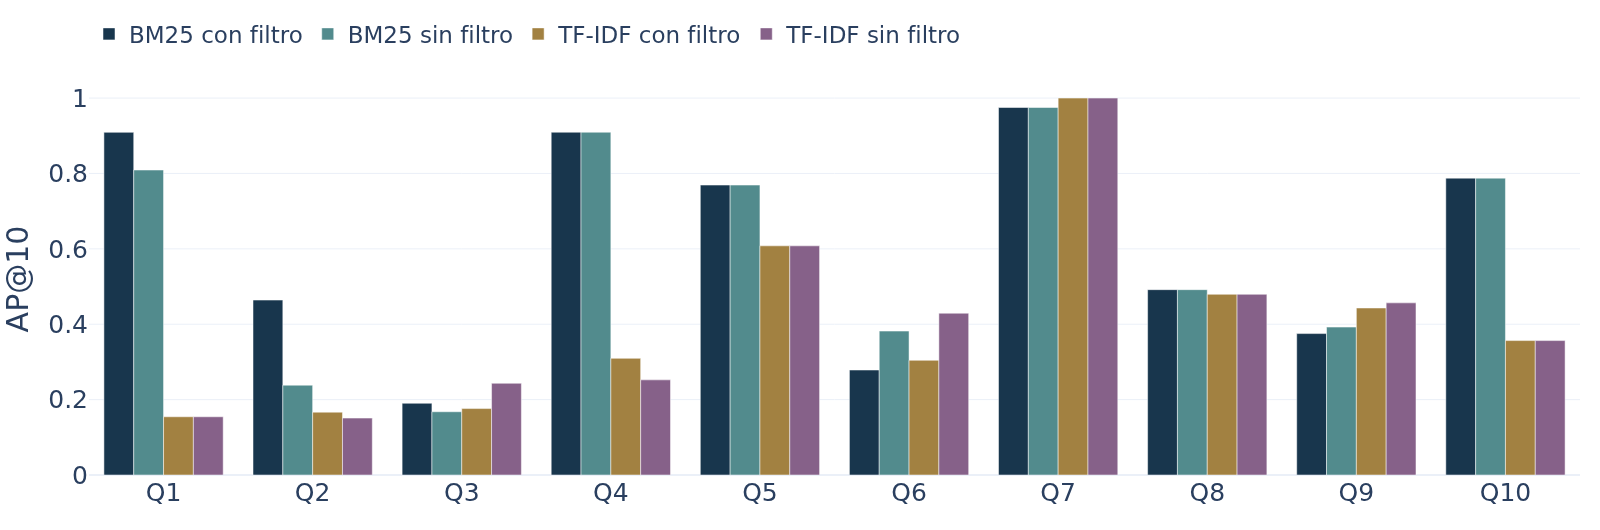
\includegraphics[width=.90\linewidth]{chart-000.png}
\caption{AP oficial por consulta para las cuatro variantes. Fuente: \texttt{salida/05\_ir\_por\_consulta.csv}.}
\end{figure}

Las ganancias no son uniformes: BM25 supera a TF--IDF en Q1 (0.9091 frente a 0.1545) y Q4 (0.9094 frente a 0.3095); TF--IDF gana en Q6 (0.3043 frente a 0.2785), Q7 (1.0000 frente a 0.9750) y Q9 (0.4431 frente a 0.3752). Q3 presenta AP bajo en ambos sistemas (0.1762 y 0.1903). Ni la longitud de las consultas (entre cuatro y seis tokens) ni un solo rasgo léxico bastan para explicar por sí solos estas diferencias.

% ====================== PÁGINA 4 ======================

\section{Extracción de entidades: reglas y BETO}
A partir de los diez pasajes mejor clasificados de cada consulta se buscaron cinco tipos de entidades: \textbf{personas (PER), organizaciones (ORG), lugares (LOC), fechas (FECHA) y montos (MONTO)}. Se combinaron dos enfoques. El primero utiliza \textbf{expresiones regulares} para localizar fechas y cantidades monetarias, y listas de nombres conocidos (\emph{gazetteers}) para reconocer organizaciones y lugares. El catálogo institucional conservó sus \textbf{76 entradas originales}: se examinaron manualmente once propuestas de ampliación, pero ninguna fue aprobada. Cuando dos reglas producen menciones superpuestas, se aplican criterios de prioridad y longitud.

El segundo enfoque emplea \textbf{BETO}, un modelo BERT para español ajustado al reconocimiento de entidades [2,3]: \texttt{mrm8488/bert-spanish-cased-finetuned-ner}, con revisión fija documentada. A diferencia de las reglas y los \emph{gazetteers}, que \textbf{detectan coincidencias mediante patrones o listas predefinidas}, BETO \textbf{predice etiquetas} PER, ORG y LOC a partir del contexto; sus intervalos se alinean con el pasaje original. La fusión integra las menciones detectadas por reglas con las entidades predichas por BETO. Cuando ambos métodos coinciden en tipo, inicio y fin, se conserva una sola entidad marcada como \emph{ambos}; los solapamientos parciales se registran por separado. \textbf{FECHA y MONTO proceden únicamente de reglas}. Los métodos quedaron fijados antes de evaluar con Gold.

\section{Gold y evaluación de extracción}
Con semilla 42 se fijaron \textbf{20 pasajes únicos}, dos por consulta. El alumno anotó \textbf{138 entidades} antes de consultar predicciones y cerró el Gold en Streamlit. El pasaje \texttt{1133\_87} fue revisado sin entidades. La coincidencia evaluada es estricta: mismo pasaje, tipo e intervalo \([\mathrm{inicio},\mathrm{fin})\). Con verdaderos positivos, falsos positivos y falsos negativos se calculan precisión, exhaustividad y F1:

\begin{equation}
P=\frac{TP}{TP+FP},\qquad R=\frac{TP}{TP+FN},\qquad F_1=\frac{2PR}{P+R}.
\end{equation}

\begin{table}[H]
\centering\tabfont
\caption{Evaluación IE oficial global sobre los 19 pasajes con entidades Gold.}
\begin{tabularx}{\linewidth}{@{}Xrrr@{}}
\toprule
\textbf{Enfoque} & \textbf{Precisión} & \textbf{Recall} & \textbf{F1}\\
\midrule
Reglas y gazetteers & 0.7245 & 0.5145 & 0.6017\\
BETO & 0.6947 & 0.6594 & 0.6766\\
\rowcolor{pale} \textbf{Combinado} & \textbf{0.6257} & \textbf{0.8116} & \textbf{0.7066}\\
\bottomrule
\end{tabularx}
\end{table}
\begin{table}[H]
\centering\tinyfont
\caption{Resultados oficiales por tipo: precisión / recall / F1.}
\begin{tabularx}{\linewidth}{@{}lXXX@{}}
\toprule
\textbf{Tipo} & \textbf{Reglas} & \textbf{BETO} & \textbf{Combinado}\\
\midrule
PER & 0.0000 / 0.0000 / 0.0000 & 0.2414 / 0.8750 / 0.3784 & 0.1591 / 0.8750 / 0.2692\\
ORG & 0.7895 / 0.4412 / 0.5660 & 0.7353 / 0.7353 / 0.7353 & 0.6829 / 0.8235 / 0.7467\\
LOC & 0.8491 / 0.6000 / 0.7031 & 0.8676 / 0.7867 / 0.8252 & 0.7952 / 0.8800 / 0.8354\\
FECHA & 1.0000 / 0.1667 / 0.2857 & 0.0000 / 0.0000 / 0.0000 & 1.0000 / 0.1667 / 0.2857\\
MONTO & 1.0000 / 1.0000 / 1.0000 & 0.0000 / 0.0000 / 0.0000 & 1.0000 / 1.0000 / 1.0000\\
\bottomrule
\end{tabularx}
\end{table}
El evaluador del kit excluye el único pasaje Gold vacío (19 de 20). La prueba complementaria incluye los veinte y contabiliza sus falsos positivos: \textbf{F1 combinado 0.7022}, frente al oficial de 0.7066. El combinado incrementa el recall a 0.8116 con una precisión menor, 0.6257. El F1 perfecto para MONTO se observó solo sobre nueve entidades y no autoriza generalizar el rendimiento.

% ====================== PÁGINA 5 ======================

\Needspace{12\baselineskip}\section{Respuestas por consulta y credibilidad}
Las tablas H8 agrupan entidades obtenidas de los diez pasajes principales de BM25 con filtro y las acompañan de identificadores, fechas y extractos verificables. \textbf{Una mención no demuestra una relación}: la presencia de una dependencia junto a una obra no acredita responsabilidad, ni una cantidad aislada constituye el costo de un proyecto.

\begin{table}[H]
\centering\tinyfont
\caption{Síntesis de las diez consultas, con evidencia y límites de interpretación. Las valoraciones humanas completas permanecen en el repositorio.}
\begin{tabularx}{\linewidth}{@{}>{\bfseries}p{8mm}p{34mm}p{31mm}X@{}}
\toprule
\textbf{ID} & \textbf{Hallazgo visible} & \textbf{Pasaje [inicio:fin]} & \textbf{Limitación del resultado}\\
\midrule
Q1 & Tren Maya; estados y participantes & \texttt{396\_23 [796:1230]} & No se recupera un monto directo y completo; varias relaciones siguen ambiguas.\\
\addlinespace[2pt]
Q2 & Vacunas; farmacéuticas y dosis & \texttt{1188\_80 [393:1022]} & Cifra extraída parcialmente y asociaciones entre actor, fecha y dosis sin confirmar.\\
\addlinespace[2pt]
Q3 & Dos Bocas; Rocío Nahle & \texttt{1787\_11 [0:259]} & No toda organización mencionada construye la refinería; presupuesto e inversión no equivalen.\\
\addlinespace[2pt]
Q4 & AIFA; Santa Lucía & \texttt{1259\_59 [0:503]} & Distinguir institución participante, constructora y cifras de costo frente a ahorros.\\
\addlinespace[2pt]
Q5 & Sembrando Vida; Veracruz & \texttt{1415\_16 [157:657]} & Menciones de estados y montos sin confirmar todas las funciones de operación.\\
\addlinespace[2pt]
Q6 & Huachicol; pérdidas de 65 mil millones & \texttt{2115\_4 [592:924]} & Mezcla de pérdidas, ahorros y otros gastos; litros y relaciones geográficas incompletos.\\
\addlinespace[2pt]
Q7 & Pensión; 2,550 pesos bimestrales & \texttt{2030\_1 [548:1131]} & Identificación incompleta de institución pagadora y fecha de aumento.\\
\addlinespace[2pt]
Q8 & Salario mínimo; aumento del 16\% & \texttt{1685\_4 [805:1161]} & Se confunden porcentajes de distinta naturaleza y faltan actores empresariales.\\
\addlinespace[2pt]
Q9 & Banco del Bienestar; 2,296 sucursales & \texttt{347\_71 [322:888]} & Sucursales previstas, construidas y operativas no deben sumarse como equivalentes.\\
\addlinespace[2pt]
Q10 & Interoceánico; Salina Cruz & \texttt{1272\_17 [0:312]} & Inversión parcial sin costo total; fecha de reporte no equivale a inauguración.\\
\bottomrule
\end{tabularx}
\end{table}

\notebox{Corrección de lectura en Q2.}{El fragmento \emph{«383 mil 375 dosis»} no debe interpretarse aisladamente como cantidad total: en la revisión de las evidencias se identificó la expresión más amplia \emph{«11 millones 383 mil 375 dosis»}. La tabla H8 original se conserva como resultado del sistema; aquí se documenta el truncamiento en lugar de validarlo.}

\vspace{2pt}
{\sffamily\fontsize{8.3}{10}\selectfont\color{teal}\textbf{BALANCE H8}\hspace{8pt}451 filas: \textbf{126} respaldadas en texto, \textbf{322} ambiguas y \textbf{3} sin evidencia suficiente.}\par
El estado \emph{respaldado en texto} indica correspondencia con el corpus, no veracidad externa. Las diez valoraciones del alumno se mantienen completas en \texttt{anotaciones/valoraciones.yaml}; no se sustituyen por inferencias redactadas automáticamente.

% ====================== PÁGINA 6 ======================

\Needspace{10\baselineskip}\section{Errores, discusión y conclusiones}
\subsection{Errores auditados en extracción}
La coincidencia estricta de spans revela errores concretos. En \texttt{1458\_12} se fragmenta \emph{Istmo de Tehuantepec} (Gold \texttt{[377:397]}); en \texttt{326\_25} se omite \emph{SEDENA} \texttt{[73:79]}. En \texttt{228\_7}, la regla marca como LOC \emph{Corredor Interoceánico del Istmo de Tehuantepec} \texttt{[340:387]}, mientras el Gold cerrado consigna ORG: la discrepancia se mantiene sin revisar retrospectivamente la anotación. En \texttt{1277\_28}, la expresión \emph{SERVIDORA DE LA NACIÓN} \texttt{[17:39]} genera un falso PER en la marca del interlocutor. Estas observaciones identifican fallas, pero no prueban que las mayúsculas sean su causa única.

El posproceso auditado \texttt{2-vacios-auditados} elimina solo spans vacíos después de recortar signos y espacios. El disparador fue una comilla predicha como LOC en \texttt{1812\_0 [945:946]}. Se conservaron las cachés originales y el estado congelado. La versión previa abortó sin F1 completo; el análisis adicional de las transformaciones reportó F1 de modelo crudo \textbf{0.5292}, recorte sin unión interpalabra \textbf{0.6667} y versión final \textbf{0.6766}, sin utilizarlos para escoger parámetros retrospectivamente.

\subsection{Discusión y conclusiones}
Para este corpus y este protocolo, \textbf{BM25 con filtro fue la mejor variante según MAP oficial}, aunque TF--IDF superó a BM25 en consultas particulares. En IE, la fusión de reglas y BETO mejoró la exhaustividad respecto a los sistemas individuales, a costa de menor precisión. La diferencia entre F1 oficial (0.7066) y complementario (0.7022) demuestra que la definición del conjunto evaluado importa incluso cuando se conserva el mismo Gold.

El límite más importante de las respuestas no es solo detectar nombres: es \textbf{vincular entidades con hechos específicos}. Un monto puede indicar costo, ahorro o presupuesto; una organización puede aparecer en un discurso sin ser responsable de la obra; una fecha del discurso puede no ser la fecha del evento. Las 322 filas ambiguas y las valoraciones humanas muestran por qué la trazabilidad debe acompañarse de cautela interpretativa. La muestra Gold de veinte pasajes y el carácter léxico de los modelos limitan la generalización.

\Needspace{9\baselineskip}\section{Reproducibilidad, autoría y referencias}
El repositorio documenta descarga del corpus, dependencias, parámetros, revisiones y hashes. En una comprobación con entorno y cachés vacíos se reconstruyeron corpus, índice y rankings, y \textbf{55 CSV coincidieron exactamente}, incluidos los seis archivos oficiales. El entorno se fija mediante \texttt{uv.lock}; el README describe los comandos para reproducir las salidas y ejecutar Streamlit.

\textbf{Uso de IA.} Claude Code y Codex asistieron en programación, pruebas, herramientas, generación de tablas y elaboración del borrador. El alumno efectuó los juicios de relevancia, la anotación Gold, la revisión de gazetteer y las valoraciones de credibilidad. Esta revisión editorial y maquetación del informe contó además con ChatGPT. Los auxiliares humanos no se sustituyeron por etiquetas generadas automáticamente.

\vspace{2pt}
{\fontsize{8.5}{10.5}\selectfont
\begin{enumerate}[leftmargin=13pt,label={[\arabic*]},itemsep=1pt,topsep=1pt]
\item Robertson, S. y Zaragoza, H. (2009). \emph{The Probabilistic Relevance Framework: BM25 and Beyond}. Foundations and Trends in Information Retrieval, 3(4), 333--389. DOI: 10.1561/1500000019.
\item Devlin, J. et al. (2019). \emph{BERT: Pre-training of Deep Bidirectional Transformers for Language Understanding}. NAACL--HLT, 4171--4186. \url{https://aclanthology.org/N19-1423/}.
\item Cañete, J. et al. (2020). \emph{Spanish Pre-Trained BERT Model and Evaluation Data}. PML4DC, ICLR.
\item carevies. \texttt{discursos\_AMLO} (Hugging Face); modelo NER \texttt{mrm8488/bert-spanish-cased-finetuned-ner}. Revisiones y contratos: README y PRD v3.0.
\end{enumerate}
}

\end{document}
